\documentclass[utf8x,xcolor=pdftex,dvipsnames,table]{beamer}
\usetheme{Malmoe}  % Now it's a beamer presentation with the lisa theme!
\setbeamertemplate{footline}[page number]
\usecolortheme{beaver}
\usepackage[T1]{fontenc}
\usepackage{amsmath}
\usepackage[utf8x]{inputenc}
%\logo{\includegraphics[width=.8in]{UdeM_NoirBleu_logo_Marie_crop}}
\usepackage{listings}

\newcommand{\superscript}[1]{\ensuremath{^{\textrm{#1}}}}

\mode<presentation>

\title{Theano and LSTM for Sentiment Analysis}

\author{%
\footnotesize
Frédéric Bastien \newline
Département d'Informatique et de Recherche Opérationnelle \newline
Université de Montréal \newline
Montréal, Canada \newline
\texttt{bastienf@iro.umontreal.ca} \newline \newline
Presentation prepared with Pierre Luc Carrier, KyungHyun Cho and \newline
 Çağlar Gülçehre
}

\date{Next.ML 2015}

\setbeamertemplate{navigation symbols}{}
\begin{document}

\begin{frame}[plain]
 \titlepage
 \vspace{-5em}
 \includegraphics[width=1in]{../hpcs2011_tutorial/pics/lisabook_logo_text_3.png}
 \hfill
 \includegraphics[width=.8in]{../hpcs2011_tutorial/pics/UdeM_NoirBleu_logo_Marie_crop}
\end{frame}

\section{Introduction}
\begin{frame}
  \frametitle{Task}

This is a classification task where we need to tell if the movie review was
positive or negative.

We use the IMDB dataset.
\end{frame}

\begin{frame}
  \tableofcontents[currentsection]
\end{frame}


\begin{frame}{High level}\setcounter{page}{1}
  Python <- \{NumPy/SciPy/libgpuarray\} <- Theano <- Pylearn2
  \begin{itemize}
  \item Python: OO coding language
  \item Numpy: $n$-dimensional array object and scientific computing toolbox
  \item SciPy: sparse matrix objects and more scientific computing functionality
  \item libgpuarray: GPU $n$-dimensional array object in C for CUDA and OpenCL
  \item Theano: compiler/symbolic graph manipulation
  \item Pylearn2: machine learning framework for researchers
  \end{itemize}
\end{frame}

%% \begin{frame}{Others}
%%   \begin{itemize}
%%   \item IPython: Advanced python shell
%%   \item IPython notebook: web-based interactive computational environment where you can combine code execution, text, mathematics, plots and rich media into a single document
%%   \item matplotlib: one of the many plotting library
%%  \item PyTables: hdf5 container with extra functionality
%%  \item pandas: other data structure
%%  \item ...
%%   \end{itemize}
%% \end{frame}

\begin{frame}{Python}
  \begin{itemize}
  \item General-purpose high-level OO interpreted language
  \item Emphasizes code readability
  \item Comprehensive standard library
  \item Dynamic type and memory management
  \item Slow execution
  \item Easily extensible with C
  \item Popular in {\em web development}\ and {\em scientific communities}
  \end{itemize}
\end{frame}

\begin{frame}{NumPy/SciPy}
  \begin{itemize}
  \item Python floats are full-fledged objects on the heap
      \begin{itemize}
      \item Not suitable for high-performance computing!
      \end{itemize}

  \item NumPy provides an $n$-dimensional numeric array in Python
      \begin{itemize}
      \item Perfect for high-performance computing
      \item Slices of arrays are views (no copying)
      \end{itemize}

  \item NumPy provides
      \begin{itemize}
      \item Elementwise computations
      \item Linear algebra, Fourier transforms
      \item Pseudorandom number generators (many distributions)
      \end{itemize}

  \item SciPy provides lots more, including
      \begin{itemize}
      \item Sparse matrices
      \item More linear algebra
      \item Solvers and optimization algorithms
      \item Matlab-compatible I/O
      \item I/O and signal processing for images and audio
      \end{itemize}
  \end{itemize}
\end{frame}

\begin{frame}{What's missing?}
  \begin{itemize}
    \item Non-lazy evaluation (required by Python) hurts performance
    \item Bound to the CPU
    \item Lacks symbolic or automatic differentiation
    \item No automatic speed and stability optimization
  \end{itemize}

\end{frame}

\begin{frame}{Goal of the stack}
\begin{center}
\begin{bf}Fast to develop\end{bf}\newline \bigskip
\begin{bf}Fast to run\end{bf}\newline \bigskip
\hspace{-2.5cm}

\includegraphics[width=0.35\textwidth]{../omlw2014/road-runner-1.jpg}
\end{center}
\end{frame}


\section{Theano}
\begin{frame}
  \tableofcontents[currentsection]
\end{frame}

\begin{frame}{Description}

  High-level domain-specific language for numeric computation.

  \begin{itemize}
    \item Syntax as close to NumPy as possible
    \item Compiles most common expressions to C for CPU and/or GPU
    \item Limited expressivity means more opportunities for optimizations
    \begin{itemize}
      \item No subroutines -> global optimization
      \item Strongly typed -> compiles to C
      \item Array oriented -> easy parallelism
      \item Support for looping and branching in expressions
    \end{itemize}
    \item Automatic speed and stability optimizations
    \item Can reuse other technologies for best performance.
    \begin{itemize}
      \item BLAS, SciPy, Cython, Numba, PyCUDA, CUDA, ...
    \end{itemize}
    \item Automatic differentiation and R op
    \item Sparse matrices (CPU only)
    \item Extensive unit-testing and self-verification
    \item Works on Linux, OS X and Windows
  \end{itemize}
\end{frame}



%% \begin{frame}{Why scripting for GPUs?}
%%   \begin{bf}They complement each other\end{bf}

%%   GPUs are everything that high level languages are not

%%   \begin{itemize}
%%     \item Highly parallel
%%     \item Very architecture-sensitive
%%     \item Built for maximum FP/memory throughput
%%     \item So hard to program that meta-programming is easier
%%   \end{itemize}

%%   \begin{bf}Best of both worlds:\end{bf} easily scripted code which invokes high-performance GPU kernels.

%%   \begin{bf}Theano C code generation removes overhead\end{bf} of
%%   function calls between Python and C by launching many C functions at once.

%% \end{frame}

\begin{frame}{Project status?}
  \begin{itemize}
    \item Mature: Theano has been developed and used since January 2008 (7 yrs old)
    \item Driven hundreds research papers
    \item Good user documentation
    \item Active mailing list with participants from outside our lab
    \item Core technology for a few Silicon-Valley start-ups
    \item Many contributors (some from outside our lab)
    \item Used to teach many university classes
    \item Has been used for research at big compagnies
  \end{itemize}
  Theano: \url{deeplearning.net/software/theano/}

  Deep Learning Tutorials: \url{deeplearning.net/tutorial/}
\end{frame}

\begin{frame}[fragile]
  \frametitle{Simple example}

\lstset{language=Python,
        commentstyle=\itshape\color{blue},
        stringstyle=\color{violet},
        }
\begin{lstlisting}
import theano
# declare symbolic variable
a = theano.tensor.vector("a")

# build symbolic expression
b = a + a ** 10

# compile function
f = theano.function([a], b)

# Execute with numerical value
print f([0, 1, 2])
# prints `array([0, 2, 1026])`
\end{lstlisting}
\end{frame}

\begin{frame}{Simple example}
\center
\includegraphics[width=0.35\textwidth]{../hpcs2011_tutorial/pics/f_unoptimized.png}
\hspace{0.1\textwidth}
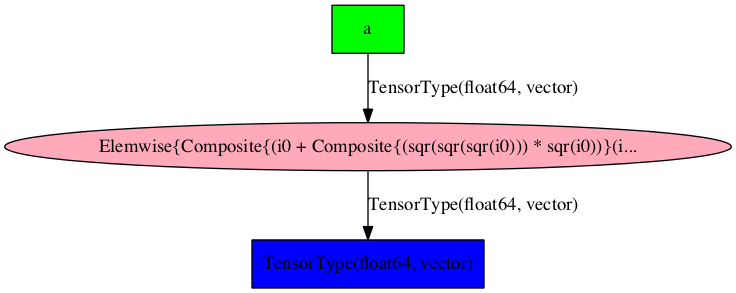
\includegraphics[width=0.35\textwidth]{../hpcs2011_tutorial/pics/f_optimized.png}
\end{frame}


%% \begin{frame}{Overview of Library}
%%   Theano is many things
%%   \begin{itemize}
%%   \item Language
%%   \item Compiler
%%   \item Python library
%%   \end{itemize}
%% \end{frame}

\begin{frame}{Overview Language}
  \begin{itemize}
  \item Operations on scalar, vector, matrix, tensor, and sparse variables
  \item Linear algebra
  \item Element-wise nonlinearities
  \item Convolution
  \item Indexing, slicing and advanced indexing.
  \item Reduction
  \item Dimshuffle (n-dim transpose)
  \item Extensible
  \end{itemize}
\end{frame}


\begin{frame}[fragile]
  \frametitle{Scalar math}
Some example of scalar operations:
\lstset{language=Python,
        commentstyle=\itshape\color{blue},
        stringstyle=\color{violet},
        }
\begin{lstlisting}
import theano
from theano import tensor as T
x = T.scalar()
y = T.scalar()
z = x+y
w = z*x
a = T.sqrt(w)
b = T.exp(a)
c = a ** b
d = T.log(c)
\end{lstlisting}
\end{frame}

\begin{frame}[fragile]
  \frametitle{Vector math}

\lstset{language=Python,
        commentstyle=\itshape\color{blue},
        stringstyle=\color{violet},
        }
\begin{lstlisting}
from theano import tensor as T
x = T.vector()
y = T.vector()
# Scalar math applied elementwise
a = x * y
# Vector dot product
b = T.dot(x, y)
# Broadcasting (as NumPy, very powerful)
c = a + b
\end{lstlisting}
\end{frame}

\begin{frame}[fragile]
  \frametitle{Matrix math}

\lstset{language=Python,
        commentstyle=\itshape\color{blue},
        stringstyle=\color{violet},
        }
\begin{lstlisting}
from theano import tensor as T
x = T.matrix()
y = T.matrix()
a = T.vector()
# Matrix-matrix product
b = T.dot(x, y)
# Matrix-vector product
c = T.dot(x, a)
\end{lstlisting}
\end{frame}

\begin{frame}[fragile]
  \frametitle{Tensors}
  Using Theano:
  \begin{itemize}
  \item Dimensionality defined by length of ``broadcastable'' argument
  \item Can add (or do other elemwise op) on two
    tensors with same dimensionality
  \item Duplicate tensors along broadcastable axes to make size match
  \end{itemize}
\lstset{language=Python,
        commentstyle=\itshape\color{blue},
        stringstyle=\color{violet},
        }
\begin{lstlisting}
from theano import tensor as T
tensor3 = T.TensorType(
    broadcastable=(False, False, False),
    dtype='float32')
x = T.tensor3()
\end{lstlisting}
\end{frame}

\begin{frame}[fragile]
  \frametitle{Reductions}
\lstset{language=Python,
        commentstyle=\itshape\color{blue},
        stringstyle=\color{violet},
        }
\begin{lstlisting}
from theano import tensor as T
tensor3 = T.TensorType(
    broadcastable=(False, False, False),
    dtype='float32')
x = tensor3()
total = x.sum()
marginals = x.sum(axis=(0, 2))
mx = x.max(axis=1)
\end{lstlisting}
\end{frame}

\begin{frame}[fragile]
  \frametitle{Dimshuffle}

\lstset{language=Python,
        commentstyle=\itshape\color{blue},
        stringstyle=\color{violet},
        }
\begin{lstlisting}
from theano import tensor as T
tensor3 = T.TensorType(
    broadcastable=(False, False, False))
x = tensor3()
y = x.dimshuffle((2, 1, 0))
a = T.matrix()
b = a.T
# Same as b
c = a.dimshuffle((0, 1))
# Adding to larger tensor
d = a.dimshuffle((0, 1, 'x'))
e = a + d
\end{lstlisting}
\end{frame}

\begin{frame}[fragile]
  \frametitle{Indexing}
  As NumPy!
  This mean all slices, index selection return view
\lstset{language=Python,
        commentstyle=\itshape\color{blue},
        stringstyle=\color{violet},
        }
\begin{lstlisting}
# return views, supported on GPU
a_tensor[int]
a_tensor[int, int]
a_tensor[start:stop:step, start:stop:step]
a_tensor[::-1] # reverse the first dimension

# Advanced indexing, return copy
a_tensor[an_index_vector] # Supported on GPU
a_tensor[an_index_vector, an_index_vector]
a_tensor[int, an_index_vector]
a_tensor[an_index_tensor, ...]
\end{lstlisting}
\end{frame}

\subsection{Compiling/Running}
\begin{frame}{Compiling and running expression}
  \begin{itemize}
  \item theano.function
  \item shared variables and updates
  \item compilation modes
  \item compilation for GPU
  \item optimizations
  \end{itemize}
\end{frame}

\begin{frame}[fragile]
  \frametitle{theano.function}

\lstset{language=Python,
        commentstyle=\itshape\color{blue},
        stringstyle=\color{violet},
        }
\begin{lstlisting}
>>> from theano import tensor as T
>>> x = T.scalar()
>>> y = T.scalar()
>>> from theano import function
>>> # first arg is list of SYMBOLIC inputs
>>> # second arg is SYMBOLIC output
>>> f = function([x, y], x + y)
>>> # Call it with NUMERICAL values
>>> # Get a NUMERICAL output
>>> f(1., 2.)
array(3.0)
\end{lstlisting}
\end{frame}

\begin{frame}{Shared variables}
  \begin{itemize}
  \item It’s hard to do much with purely functional programming
  \item ``shared variables'' add just a little bit of imperative programming
  \item A ``shared variable'' is a buffer that stores a numerical value for a Theano variable
  \item Can write to as many shared variables as you want, once each, at the end of the function
  \item  Modify outside Theano function with get\_value() and set\_value() methods.
  \end{itemize}
\end{frame}

\begin{frame}[fragile]
  \frametitle{Shared variable example}

\lstset{language=Python,
        commentstyle=\itshape\color{blue},
        stringstyle=\color{violet},
        }
\begin{lstlisting}
>>> from theano import shared
>>> x = shared(0.)
>>> from theano.compat.python2x import OrderedDict
>>> updates = OrderedDict()
>>> updates[x] = x + 1
>>> f = function([], updates=updates)
>>> f()
>>> x.get_value()
1.0
>>> x.set_value(100.)
>>> f()
>>> x.get_value()
101.0
\end{lstlisting}
\end{frame}

\begin{frame}{Which dict?}
  \begin{itemize}
  \item Use theano.compat.python2x.OrderedDict
  \item Not collections.OrderedDict
  \begin{itemize}
  \item This isn’t available in older versions of python
  \end{itemize}
  \item Not \{\} aka dict
  \begin{itemize}
  \item The iteration order of this built-in class is not
    deterministic (thanks, Python!) so if Theano
    accepted this, the same script could compile
    different C programs each time you run it
  \end{itemize}
  \end{itemize}
\end{frame}

\begin{frame}{Compilation modes}
  \begin{itemize}
  \item Can compile in different modes to get different kinds of programs
  \item Can specify these modes very precisely with arguments to theano.function
  \item Can use a few quick presets with environment variable flags
  \end{itemize}
\end{frame}

\begin{frame}{Example preset compilation modes}
  \begin{itemize}
  \item FAST\_RUN: default. Fastest execution, slowest compilation
  \item FAST\_COMPILE: Fastest compilation, slowest execution. No C code.
  \item DEBUG\_MODE: Adds lots of checks.
Raises error messages in situations other
modes regard as fine.
  \item optimizer=fast\_compile: as mode=FAST\_COMPILE, but with C code.
  \item theano.function(..., mode=``FAST\_COMPILE'')
  \item THEANO\_FLAGS=mode=FAST\_COMPILE python script.py
  \end{itemize}
\end{frame}

\begin{frame}{Compilation for GPU}
  \begin{itemize}
  \item Theano current back-end only supports 32 bit on GPU
  \item libgpuarray (new-backend) support all dtype
  \item CUDA supports 64 bit, but is slow on gamer GPUs
  \item T.fscalar, T.fvector, T.fmatrix are all 32 bit
  \item T.scalar, T.vector, T.matrix resolve to 32 bit or 64 bit depending on theano’s floatX flag
  \item floatX is float64 by default, set it to float32
  \item Set device flag to gpu (or a specific gpu, like gpu0)
  \item Flag: warn\_float64={'ignore', 'warn', 'raise', 'pdb'}
  \end{itemize}
\end{frame}

\subsection{Modifying expressions}
\begin{frame}{Modifying expressions}
  \begin{itemize}
  \item The grad method
  \item Others

%  \item Variable nodes
%  \item Types
%  \item Ops
%  \item Apply nodes
  \end{itemize}
\end{frame}

\begin{frame}[fragile]
  \frametitle{The grad method}

\lstset{language=Python,
        commentstyle=\itshape\color{blue},
        stringstyle=\color{violet},
        }
\begin{lstlisting}
>>> x = T.scalar('x')
>>> y = 2. * x
>>> g = T.grad(y, x)
# Print the not optimized graph
>>> theano.printing.debugprint(g)
Elemwise{mul} [@A] ''
 |Elemwise{second,no_inplace} [@B] ''
 | |Elemwise{mul,no_inplace} [@C] ''
 | | |TensorConstant{2.0} [@D]
 | | |x [@E]
 | |TensorConstant{1.0} [@F]
 |TensorConstant{2.0} [@D]
\end{lstlisting}
\end{frame}

%% \begin{frame}{Theano Variables}
%%   \begin{itemize}
%%   \item A Variable is a theano expression
%%   \item Can come from T.scalar, T.matrix, etc.
%%   \item Can come from doing operations on other Variables
%%   \item Every Variable has a type field, identifying its Type \newline
%%     e.g. TensorType((True, False), ‘float32’)
%%   \item Variables can be thought of as nodes in a graph
%%   \end{itemize}
%% \end{frame}

%% \begin{frame}{Ops}

%%   \begin{itemize}
%%   \item  An Op is any class that describes a
%% mathematical function of some variables
%%   \item Can call the op on some variables to get a
%% new variable or variables
%%   \item An Op class can supply other forms of
%% information about the function, such as its
%% derivatives
%%   \end{itemize}
%% \end{frame}

%% \begin{frame}{Apply nodes}
%%   \begin{itemize}
%%   \item The Apply class is a specific instance of an application of an Op
%%   \item Notable fields:
%%     \begin{itemize}
%%     \item op: The Op to be applied
%%     \item inputs: The Variables to be used as input
%%     \item outputs: The Variables produced
%%     \end{itemize}
%%   \item Variable.owner identifies the Apply that created the variable
%%   \item Variable and Apply instances are nodes and owner/
%%     inputs/outputs identify edges in a Theano graph
%%   \end{itemize}
%% \end{frame}

\begin{frame}{Others}
  \begin{itemize}
  \item R\_op, L\_op for hessian free
  \item hessian
  \item jacobian
  \item you can navigate the graph if you need
      (go from the result of computation to its input, recursively)
  \end{itemize}
\end{frame}

\subsection{Debugging}
\begin{frame}{Debugging}
  \begin{itemize}
  \item DEBUG\_MODE
  \item Error message
  \item theano.printing.debugprint
  \end{itemize}
\end{frame}

\begin{frame}[fragile]
  \frametitle{Error message: code}
\lstset{language=Python,
        commentstyle=\itshape\color{blue},
        stringstyle=\color{violet},
        }
\begin{lstlisting}
import numpy as np
import theano
import theano.tensor as T
x = T.vector()
y = T.vector()
z = x + x
z = z + y
f = theano.function([x, y], z)
f(np.ones((2,)), np.ones((3,)))
\end{lstlisting}
\end{frame}

\begin{frame}[fragile]
  \frametitle{Error message: 1st part}

\lstset{language=Python,
        commentstyle=\itshape\color{blue},
        stringstyle=\color{violet},
        basicstyle=\scriptsize
        }
\begin{lstlisting}
Traceback (most recent call last):
[...]
ValueError: Input dimension mis-match.
    (input[0].shape[0] = 3, input[1].shape[0] = 2)
Apply node that caused the error:
   Elemwise{add,no_inplace}(<TensorType(float64, vector)>,
                            <TensorType(float64, vector)>,
                            <TensorType(float64, vector)>)
Inputs types: [TensorType(float64, vector),
               TensorType(float64, vector),
               TensorType(float64, vector)]
Inputs shapes: [(3,), (2,), (2,)]
Inputs strides: [(8,), (8,), (8,)]
Inputs scalar values: ['not scalar', 'not scalar', 'not scalar']
\end{lstlisting}
\end{frame}

\begin{frame}[fragile]
  \frametitle{Error message: 2st part}

\lstset{language=Python,
        commentstyle=\itshape\color{blue},
        stringstyle=\color{violet},
        basicstyle=\footnotesize
        }
\begin{lstlisting}
HINT: Re-running with most Theano optimization
disabled could give you a back-traces when this
node was created. This can be done with by setting
the Theano flags optimizer=fast_compile
HINT: Use the Theano flag 'exception_verbosity=high'
for a debugprint of this apply node.
\end{lstlisting}
\end{frame}

\begin{frame}[fragile]
  \frametitle{Error message: exception\_verbosity=high}

\lstset{language=Python,
        commentstyle=\itshape\color{blue},
        stringstyle=\color{violet},
        basicstyle=\scriptsize,
        xleftmargin=-1em
        }
\begin{lstlisting}
Debugprint of the apply node:
Elemwise{add,no_inplace} [@A] <TensorType(float64, vector)> ''
 |<TensorType(float64, vector)> [@B] <TensorType(float64, vector)>
 |<TensorType(float64, vector)> [@C] <TensorType(float64, vector)>
 |<TensorType(float64, vector)> [@C] <TensorType(float64, vector)>
\end{lstlisting}
\end{frame}

\begin{frame}[fragile]
  \frametitle{Error message: optimizer=fast\_compile}

\lstset{language=Python,
        commentstyle=\itshape\color{blue},
        stringstyle=\color{violet},
        }
\begin{lstlisting}
Backtrace when the node is created:
  File "test.py", line 7, in <module>
    z = z + y

\end{lstlisting}
\end{frame}

\begin{frame}[fragile]
  \frametitle{Error message: Traceback}

\lstset{language=Python,
        commentstyle=\itshape\color{blue},
        stringstyle=\color{violet},
        basicstyle=\footnotesize,
        xleftmargin=-1em
        }
\begin{lstlisting}
Traceback (most recent call last):
  File "test.py", line 9, in <module>
    f(np.ones((2,)), np.ones((3,)))
  File "/u/bastienf/repos/theano/compile/function_module.py",
       line 589, in __call__
    self.fn.thunks[self.fn.position_of_error])
  File "/u/bastienf/repos/theano/compile/function_module.py",
       line 579, in __call__
    outputs = self.fn()

\end{lstlisting}
\end{frame}

\begin{frame}[fragile]
  \frametitle{debugprint}

\lstset{language=Python,
        commentstyle=\itshape\color{blue},
        stringstyle=\color{violet},
        }
\begin{lstlisting}
>>> from theano.printing import debugprint
>>> debugprint(a)
Elemwise{mul,no_inplace} [@A] ''
 |TensorConstant{2.0} [@B]
 |Elemwise{add,no_inplace} [@C] 'z'
   |<TensorType(float64, scalar)> [@D]
   |<TensorType(float64, scalar)> [@E]
\end{lstlisting}
\end{frame}

%% \begin{frame}{Pylearn2}

%%   Machine Learning library aimed at researchers

%%   \begin{itemize}
%%     \item Built on top of Theano, for fast execution and use of GPU
%%     \item Easy to try variants of implemented algorithms, and to extend them (using Theano)
%%     \item Very modular, each component of the library can be used in isolation
%%     \item Experiments can be specified through a YAML config file, or by a Python script
%%     \item Scripts for visualizing weights, plot monitored values
%%   \end{itemize}
%% \end{frame}


%% \begin{frame}{libgpuarray}
%%   Goal: A common GPU $n$-dimensional array that can be reused by all projects, support for both CUDA and OpenCL.
%%   \newline \newline
%%   Motivation:
%%   \begin{itemize}
%%   \item Currently there are at least 6 different GPU arrays in Python
%%     \begin{itemize}
%%     \item CudaNdarray (Theano), GPUArray (pycuda), CUDAMatrix (cudamat), GPUArray (pyopencl), Clyther, Copperhead, ...
%%     \item There are even more if we include other languages.
%%     \end{itemize}
%%   \item They are incompatible
%%     \begin{itemize}
%%     \item None have the same properties and interface
%%     \end{itemize}
%%   \item All of them implement a subset of numpy.ndarray properties
%%   \item This is the new GPU backend on Theano
%%   \end{itemize}
%% \end{frame}


%% \begin{frame}{Project status?}
%%   \begin{itemize}
%%   \item Usable directly, but not all implementation available.
%%   \item Multiple GPUs works.
%%   \item Is the next GPU array container for Theano and is working.
%%     \begin{itemize}
%%     \item Not all Theano implementations available now.
%%     \item OpenCL misses more implementations.
%%     \item Multiple GPUs: supported in libgpuarray
%%     \item Multiple GPUs: close to get integrated in Theano.
%%     \end{itemize}
%%   \item Web site: \url{http://deeplearning.net/software/libgpuarray/}
%%   \end{itemize}
%% \end{frame}

%% \section{libgpuarray}
%% \begin{frame}
%%   \tableofcontents[currentsection]
%% \end{frame}
%% %TODO, make much shorter
%% \begin{frame}{libgpuarray: Design Goals}
%%   \begin{itemize}
%%   \item Have the base object in C to allow collaboration with more projects.
%%     \begin{itemize}
%%     \item We want people from C, C++, ruby, R, \ldots all use the same base GPU ndarray.
%%     \end{itemize}
%%   \item Be compatible with CUDA and OpenCL.
%%   \item Not too simple, (don’t support just matrix).
%%   \item Support all dtype.
%%   \item Allow strided views.
%%   \item But still easy to develop new code that support only a few memory layout.
%%     \begin{itemize}
%%     \item This ease the development of new code.
%%     \end{itemize}
%%   \end{itemize}
%% \end{frame}

\subsection{Scan}
\begin{frame}
  \frametitle{Scan}
\begin{itemize}
\item Allows looping (for, map, while)
\item Allows recursion (reduce)
\item Allows recursion with dependency on many of the previous time steps
\item Optimize some cases like moving computation outside of scan
\item The Scan grad is done via Backpropagation Through Time(BPTT)
\end{itemize}
\end{frame}

\begin{frame}{When not to use scan}
\begin{itemize}
\item If you only need it for ``vectorization'' or
  ``broadcasting''. tensor and numpy.ndarray support them
  natively. This will be much better for that use case.

\item If you do a fixed number of iteration that is very small (2,3). You
  are probably better to just unroll the graph to do it.

\end{itemize}
\end{frame}


\begin{frame}[fragile,allowframebreaks]
  \frametitle{Scan Example1: Computing tanh(v.dot(W) + b) * d where b is binomial}

\lstset{language=Python,
        commentstyle=\itshape\color{blue},
        stringstyle=\color{violet},
        basicstyle=\footnotesize
        }
\begin{lstlisting}
import theano
import theano.tensor as T
import numpy as np

# define tensor variables
W = T.matrix("W")
X = T.matrix("X")
b_sym = T.vector("b_sym")

# define shared random stream
trng = T.shared_randomstreams.RandomStreams(1234)
d=trng.binomial(size=W[1].shape)
\end{lstlisting}
\end{frame}


\begin{frame}[fragile]
  \frametitle{Scan Example1: Computing tanh(v.dot(W) + b) * d where d is binomial (2)}

\lstset{language=Python,
        commentstyle=\itshape\color{blue},
        stringstyle=\color{violet},
        }
\begin{lstlisting}
results, updates = theano.scan(
    lambda v: T.tanh(T.dot(v, W) + b_sym) * d,
    sequences=X)
f = theano.function(inputs=[X, W, b_sym],
                    outputs=[results],
                    updates=updates)
x = np.eye(10, 2, dtype=theano.config.floatX)
w = np.ones((2, 2), dtype=theano.config.floatX)
b = np.ones((2), dtype=theano.config.floatX)

print f(x, w, b)
\end{lstlisting}
\end{frame}

\begin{frame}[fragile]
  \frametitle{Scan Example2: Computing pow(A, k)}

\lstset{language=Python,
        commentstyle=\itshape\color{blue},
        stringstyle=\color{violet},
        }
\begin{lstlisting}
import theano
import theano.tensor as T
theano.config.warn.subtensor_merge_bug = False

k = T.iscalar("k")
A = T.vector("A")

def inner_fct(prior_result, B):
    return prior_result * B
\end{lstlisting}
\end{frame}

\begin{frame}[fragile]
  \frametitle{Scan Example2: Computing pow(A, k) (2)}

\lstset{language=Python,
        commentstyle=\itshape\color{blue},
        stringstyle=\color{violet},
        }
\begin{lstlisting}
result, updates = theano.scan(
    fn=inner_fct,
    outputs_info=T.ones_like(A),
    non_sequences=A, n_steps=k)

# Scan provide us with A ** 1 through A ** k.
# Keep only the last value. Scan optimize memory.
final = result[-1]

power = theano.function(inputs=[A, k], outputs=final,
                      updates=updates)
print power(range(10), 2)
#[  0.   1.   4.   9.  16.  25.  36.  49.  64.  81.]
\end{lstlisting}
\end{frame}

\begin{frame}[fragile]
  \frametitle{Scan signature}

\lstset{language=Python,
        commentstyle=\itshape\color{blue},
        stringstyle=\color{violet},
        }
\begin{lstlisting}
result, updates = theano.scan(
    fn=inner_fct,
    sequences=[]
    outputs_info=[T.ones_like(A)],
    non_sequences=A,
    n_steps=k)
\end{lstlisting}

\begin{itemize}
\item Updates are needed if there are random numbers generated in the inner function
\begin{itemize}
\item Pass them to the call theano.function(..., updates=updates)
\end{itemize}
\item The inner function of scan takes arguments like this:
   scan: sequences, outputs\_info, non sequences
\end{itemize}

\end{frame}


\section{RNN}
\begin{frame}
  \tableofcontents[currentsection]
\end{frame}

\begin{frame}
  \frametitle{Recurrent Neural Network Overview}
\begin{itemize}
\item RNN is a class of neural network that allows to work with sequences of variable sizes.
\item It does so, by reusing weights for each element of the sequence.
\item One layer have recurrent connection to itself with a time delay.
  \begin{itemize}
  \item This create an internal state that allows to exhibit dynamic temporal behavior.
  \end{itemize}
\end{itemize}
Image from wikipedia by Fyedernoggersnodden
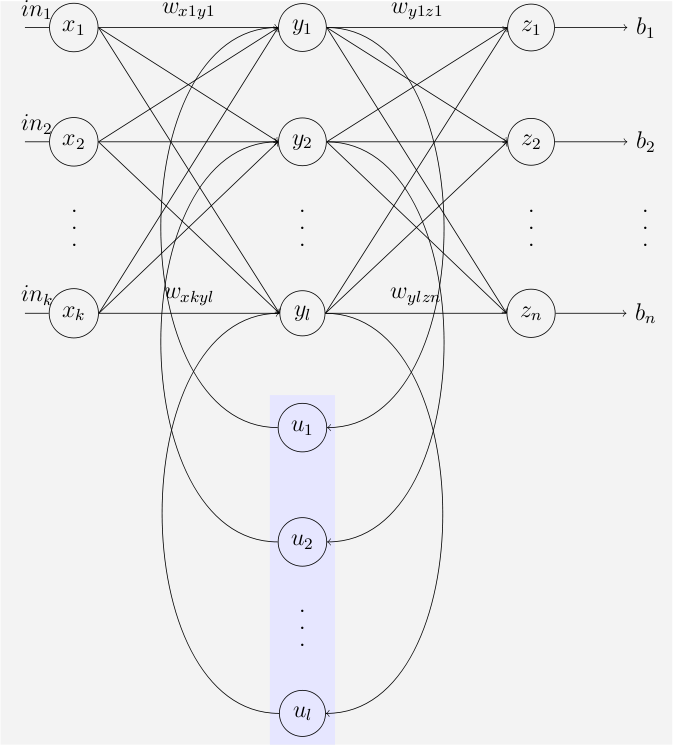
\includegraphics[width=0.35\textwidth]{../images/Elman_srnn.png}
\end{frame}

\section{LSTM}
\begin{frame}
  \tableofcontents[currentsection]
\end{frame}

\begin{frame}
  \frametitle{Motivation}
RNN gradient signal end up being multiplied a large number of times (as many as the number of timesteps).
This means that, the magnitude of the weights in the transition matrix can have a strong impact on the learning process.
\begin{itemize}
\item \begin{bf}vanishing gradients\end{bf}
 If the weights in this matrix are small (or, more formally, if the leading eigenvalue of the weight matrix is smaller than 1.0).
\item \begin{bf}exploding gradients\end{bf} If the weights in this matrix are large (or, again, more formally, if the leading eigenvalue of the weight matrix is larger than 1.0),
\end{itemize}
\end{frame}

\begin{frame}
  \frametitle{History}
\begin{itemize}
\item Original version introduced in 1997 by Hochreiter, S., \& Schmidhuber, J.
\item Forget gate introduced in 2000 by Gers, F. A., Schmidhuber, J., \& Cummins, F.
\item All people we know use forget gate now.
\end{itemize}
\end{frame}

\begin{frame}
  \frametitle{LSTM overview}
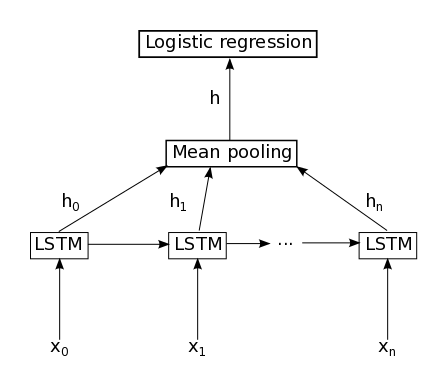
\includegraphics[width=0.75\textwidth]{../images/lstm.png}
\end{frame}


\begin{frame}
  \frametitle{LSTM cell}
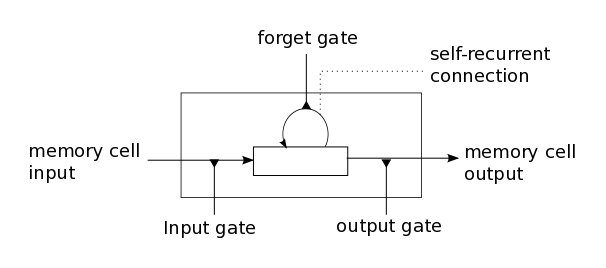
\includegraphics[width=0.75\textwidth]{../images/lstm_memorycell.png}
\end{frame}

\begin{frame}[allowframebreaks]
  \frametitle{LSTM math}
The equations on the next slide describe how a layer of memory cells is updated at every timestep t.

In these equations :

% 'm' has no special meaning here except being a size reference for the length of the label (and the spacing before the descriptions
\begin{description}[m]
\item[$x_t$] \hfill \\
is the input to the memory cell layer at time t
\item[$W_i$, $W_f$, $W_c$, $W_o$, $U_i$, $U_f$, $U_c$, $U_o$ and $V_o$] \hfill \\
 are weight matrices
\item[$b_i$, $b_f$, $b_c$ and $b_o$] \hfill \\
are bias vectors
\end{description}

\framebreak

First, we compute the values for $i_t$, the input gate, and $\widetilde{C_t}$ the candidate value for the states of the memory cells at time t :

\begin{equation}
i_t = \sigma(W_i x_t + U_i h_{t-1} + b_i)
\end{equation}
\begin{equation}
\widetilde{C_t} = tanh(W_c x_t + U_c h_{t-1} + b_c)
\end{equation}

Second, we compute the value for $f_t$, the activation of the memory cells’ forget gates at time t :

\begin{equation}
f_t = \sigma(W_f x_t + U_f h_{t-1} + b_f)
\end{equation}

\framebreak

Given the value of the input gate activation $i_t$, the forget gate activation $f_t$ and the candidate state value $\widetilde{C_t}$, we can compute $C_t$ the memory cells’ new state at time $t$ :

\begin{equation}
C_t = i_t * \widetilde{C_t} + f_t * C_{t-1}
\end{equation}

With the new state of the memory cells, we can compute the value of their output gates and, subsequently, their outputs :

\begin{equation}
o_t = \sigma(W_o x_t + U_o h_{t-1} + V_o C_t + b_1)
\end{equation}
\begin{equation}
h_t = o_t * tanh(C_t)
\end{equation}

\end{frame}

\begin{frame}
  \frametitle{Tutorial LSTM}
The model we used in this tutorial is a variation of the standard LSTM model. In this variant, the activation of a cell’s output gate does not depend on the memory cell’s state $C_t$. This allows us to perform part of the computation more efficiently (see the implementation note, below, for details). This means that, in the variant we have implemented, there is no matrix $V_o$ and equation (5) is replaced by equation (7) :

\begin{equation}
o_t = \sigma(W_o x_t + U_o h_{t-1} + b_1)
\end{equation}

\end{frame}

\begin{frame}
  \frametitle{Implementation Note}
In the code included this tutorial, the equations (1), (2), (3) and (7) are performed in parallel to make the computation more efficient. This is possible because none of these equations rely on a result produced by the other ones. It is achieved by concatenating the four matrices $W_*$ into a single weight matrix W and performing the same concatenation on the weight matrices $U_*$ to produce the matrix U and the bias vectors $b_*$ to produce the vector b. Then, the pre-nonlinearity activations can be computed with :
\vspace{-1em}
\begin{equation*}
z = \sigma(W x_t + U h_{t-1} + b)
\end{equation*}
\vspace{-2em} % don't remove the blank line

The result is then sliced to obtain the pre-nonlinearity activations for i, f, $\widetilde{C_t}$, and o and the non-linearities are then applied independently for each.
\end{frame}

\begin{frame}{LSTM Tips For Training}
\begin{itemize}
\item Do not use SGD, but use something like adagrad or rmsprop.
\item Initialize any recurrent weights as orthogonal matrices (orth\_weights). This helps optimization.
\item Take out any operation that does not have to be inside "scan".
      Theano does many cases, but not all.
\item Rescale (clip) the L2 norm of the gradient, if necessary.
\item You can use weight noise (try first with $dot(U_c+noise, h_{t-1})$).
\item You can use dropout at the output of the recurrent layer.
\end{itemize}
\end{frame}

\section{Exercices}
\begin{frame}{Exercices}
\begin{itemize}
  \item Theano exercice: Work through the ``0[1-4]*'' exercices (directory):

    Available at ``git~clone~https://github.com/abergeron/ccw\_tutorial\_theano.git''.

  \item Scan exercices: \url{http://deeplearning.net/software/theano/tutorial/loop.html\#exercise}

  \item Modif LSTM: Add the V\_o parameter and use it.
  \item Modif LSTM: Reverse the input sequence and try it like that:
        Sutskever-NIPS2014 (No solutions provided)
  \item Modif LSTM: Add to have 2 LSTM layers. The new one take the
    input in the reverse order. Then you concatenate the mean of the
    outputs of both LSTM to the logistic regression. (No solutions provided)
\end{itemize}

% I don't know how to fix this frame since it seems incomplete.

Deep Learning Tutorial on LSTM: \url{http://deeplearning.net/tutorial/lstm.html}

(It have the papers
\end{frame}


\begin{frame}{Acknowledgments}
\begin{itemize}
\item All people working or having worked at the LISA lab.
\item All Theano users/contributors
\item Compute Canada, RQCHP, NSERC, and Canada Research Chairs for providing funds or access to compute resources.
\end{itemize}
\end{frame}

\begin{frame}
\begin{center}
\Huge
Questions?
\end{center}
\end{frame}


\end{document}
